\ProvidesFile{ap-graphics.tex}[2021-01-04 graphics appendix]

\begin{VerbatimOut}{z.out}
\chapter{GRAPHICS}

There are many ways to make graphics for \LaTeX.
I like to use a system that uses \LaTeX\ fonts
so the appearance of the output is more professional.
\end{VerbatimOut}

\MyIOT


\begin{VerbatimOut}{z.out}

\section{Mathematica (Wolfram)}
\end{VerbatimOut}

\MyIOT


\begin{VerbatimOut}{z.out}

\section{MATLAB}
\end{VerbatimOut}

\MyIOT


\begin{VerbatimOut}{z.out}

\section{\METAPOST\ (uses \LaTeX\ fonts)}

I did this \METAPOST\ \cite{metapost} example
for Yanghyun Kim \cite{kim2009}.
\end{VerbatimOut}

\MyIOT


\begin{VerbatimOut}{z.out}

\newpage

\begin{figure}[ht]
  \centering 
    \subcaptionbox
      {\bfseries gr-kim1.pdf}%
      {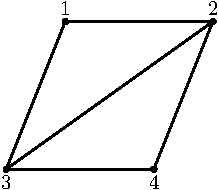
\includegraphics{gr-kim1.pdf}}%
    \vskip 0.1truein
    \subcaptionbox
      {\bfseries gr-kim2.pdf}%
      {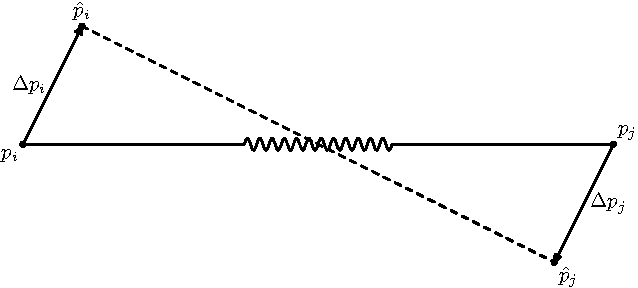
\includegraphics{gr-kim2.pdf}}%
    \caption{Graphics answers for Yanghyun Kim.}
\end{figure}
\end{VerbatimOut}

\MyIO


\begin{VerbatimOut}{z.out}

\section{R}
\end{VerbatimOut}

\MyIOT


\begin{VerbatimOut}{z.out}

\section{\TikZ\ and PGF (uses \LaTeX\ fonts)}
\end{VerbatimOut}

\MyIOT


\begin{VerbatimOut}{z.out}

\subsection{Clock}
\end{VerbatimOut}

\MyIOT


\begin{VerbatimOut}{z.out}

\begin{figure}[ht]
  \hbox to\textwidth{%
    \hfil
    \begin{tikzpicture}
      \def\CenterRadius{0.04cm}
      \def\InnerTickRadius{3.6cm}
      \def\OuterTickRadius{3.8cm}
      % Make \LR be an abbreviation for \LabelRadius so the
      % lines below will fit within the width of the page.
      \def\LabelRadius{4.5cm}      \let\LR=\LabelRadius
      \def\HourHandRadius{2.5cm}   \def\HourHandBase{0.3cm}
      \def\MinuteHandRadius{3cm}   \def\MinuteHandBase{0.4cm}
      \def\SecondHandRadius{3.5cm} \def\SecondHandBase{0.5cm}
      \def\DS{\displaystyle}
      \fill (0,0) circle (\CenterRadius);
      \foreach \i in {0,30,...,330}
      \draw (\i:\InnerTickRadius)--(\i:\OuterTickRadius);
      \node at (  0:\LR) {$\DS \qquad \sqrt9 + 9 - 9$};        %  3
      \node at ( 30:\LR) {$\DS \frac{9+9}9$};                  %  2
      \node at ( 60:\LR) {$\DS \frac{\sqrt9\sqrt9}9$};         %  1
      \node at ( 90:\LR) {$\DS 9 + \frac9{\sqrt9}$};           % 12
      \node at (120:\LR) {$\DS \frac{99}9$};                   % 11
      \node at (150:\LR) {$\DS 9 + \frac99$};                  % 10
      \node at (180:\LR) {$\DS \sqrt[\scriptstyle 9]{9^9}$};   %  9
      \node at (210:\LR) {$\DS 9 - \frac99$};                  %  8
      \node at (240:\LR) {$\DS 9 - \sqrt9 + \lceil.9\rceil$};  %  7
      \node at (270:\LR) {$\DS 9 - \frac9{\sqrt9}$};           %  6
      \node at (300:\LR) {$\DS \sqrt9\,! - \frac99$};          %  5
      \node at (330:\LR) {$\DS \sqrt9 + \frac99$};             %  4
      % In the following
      %   ABBREVIATION    DESCRIPTION
      %   deg             degrees
      %   min             minutes
      %   sec             seconds
      % for second hand:
      %   (9 sec/60 sec) * 360 deg = 54 deg;
      %   90 deg - 54 deg = 36 deg
      \draw[rotate around={36:(0,0)}]
        (-\SecondHandBase,\SecondHandBase) -- (\SecondHandRadius,0)
          -- (-\SecondHandBase,-\SecondHandBase) -- cycle;
      % for minute hand:
      %   (9 min/60 min) * 360 deg = 54 deg;
      %   90 deg - 54 deg = 36 deg
     \draw[rotate around={36:(0,0)}]
       (-\MinuteHandBase,\MinuteHandBase) -- (\MinuteHandRadius,0)
         -- (-\MinuteHandBase,-\MinuteHandBase) -- cycle;
      % for hour hand:
      %   (9 min * (60 sec/1 min)) + 9 sec) / 3600 sec
      %     = 549 sec / 3600 sec = 0.1525
      %   The hour hand is 0.1525 of the way from 9:00 to 10:00.
      %   Each hour is 30 degrees on the clock, so the hour hand
      %   position is
      %     30 deg * 0.1525 = 4.575 deg past 9:00
      %   180 deg - 4.575 deg = 175.425 deg
     \draw[rotate around={175.425:(0,0)}]
       (-\HourHandBase,\HourHandBase) -- (\HourHandRadius,0)
         -- (-\HourHandBase,-\HourHandBase) -- cycle;
    \end{tikzpicture}
    %    To make a one page clock document delete everything
    % below and add
    %     \end{document}
    \hfil
  }
  \caption{%
    The idea for this clock was originally from a
    Google+ posting by Afamefuna ``Ferdy'' Ibeabuchia.%
  }  
\end{figure}
\end{VerbatimOut}

\MyIOS


\begin{VerbatimOut}{z.out}

\subsection{Glider}
\end{VerbatimOut}

\MyIOT


\begin{VerbatimOut}{z.out}
  
\begin{figure}[ht]
  \hbox to\textwidth{%
    \hfil
    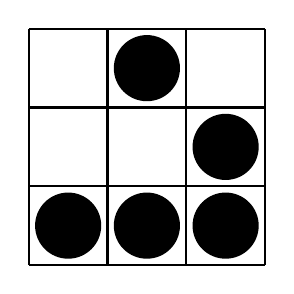
\begin{tikzpicture}[thick]
      \draw (0,0) grid (3,3);
      \foreach \c in {(0,0), (1,0), (2,0), (2,1), (1,2)}
        \fill \c + (0.5,0.5) circle (0.42);
    \end{tikzpicture}
    \hfil
  }
  \caption
  [%
    The glider
    is a pattern from the Game of Life,
    and it's used as an emblem representing the hacker community.%
  ]
  {%
    The glider \cite{hirzel2012}
    is a pattern from the Game of Life,
    and it's used as an emblem representing the hacker community.%
  }
\end{figure}
\end{VerbatimOut}

\MyIO
